\section{倒立振子のモデリング}
実験目的を達成する制御システムを設計するためにまず、倒立振子系について、状態方程式と観測方程式から成る数式モデルを導出する。
\subsection{状態方程式}
	\begin{figure}[H]
		\centering
		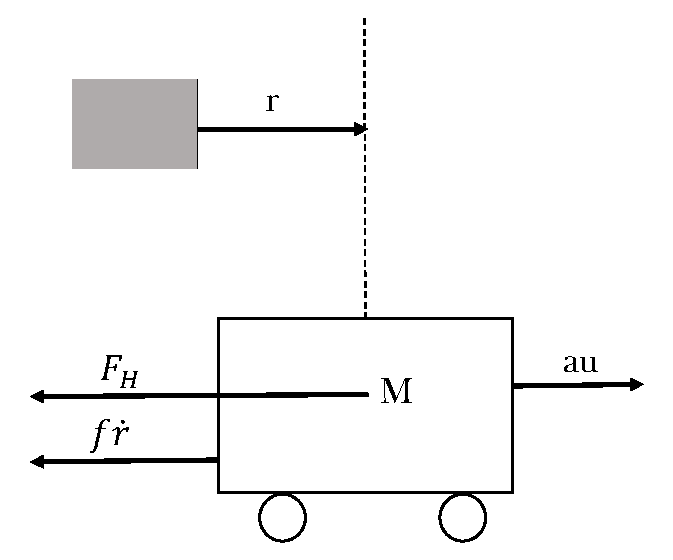
\includegraphics[width=0.4\linewidth]{gazo/cart.eps}
		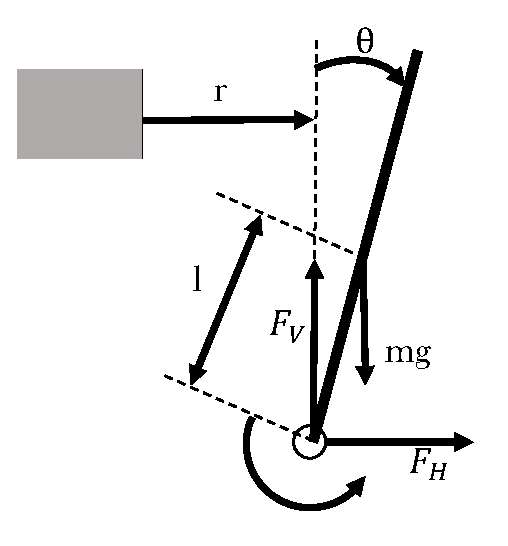
\includegraphics[width=0.4\linewidth]{gazo/stick.eps}
		\caption{数式モデル導出のための参考図}
		\label{image:reference}
	\end{figure}	
	図\ref{image:reference}を参考に各運動方程式を導出すると、\\
	台車の運動方程式は\\
	
	\begin{equation}
		M\ddot{r}=au-F_{H}-f\dot{r}
		\label{eq:motion_eq_cart}
	\end{equation}
	\\
	倒立振子の回転の運動方程式は\\
	
	\begin{equation}
		J\ddot{\theta}=lF_{V}\sin \theta -lF_{H}\cos \theta -c\dot{\theta}
		\label{eq:rotemotion_eq_stick}
	\end{equation}
	\\
	倒立振子の水平方向の運動方程式は\\
	
	\begin{equation}
		m\frac{d^{2}}{dt^{2}}(r+l\sin\theta) = F_{H}
		\label{eq:horizonmotion_eq_stick}
	\end{equation}
	\\
	倒立振子の垂直方向の運動方程式は\\
	
	\begin{equation}
		m\frac{d^{2}}{dt^{2}}(l\cos\theta) = F_{V}-mg
		\label{eq:vertical_eq_stick}
	\end{equation}
	
	となる。
	\par
	ここで各式の導出過程を述べる。図\ref{image:reference}より台車の運動方程式は、振り子からの水平抗力$F_{H}$を考慮してニュートンの第二法則より(\ref{eq:motion_eq_cart})
	式を導くことができる。
	ただし、$M$は台車の質量、$f$は台車の摩擦係数、$a$は駆動アンプへの入力電圧から台車への駆動までのゲイン、$u$はモータの駆動アンプへの入力電圧、$r$は台車の基準位置からの変位である。
	同様にニュートンの第二法則を用いることで(\ref{eq:horizonmotion_eq_stick}),(\ref{eq:vertical_eq_stick})式の運動方程式を導くことができる。
	ただし、$m$は振り子の質量、$l$は回転軸・重心間の距離、$g$は重力加速度、$F_{V}$は振り子が台車から受ける垂直抗力である。
	また、$\theta$は鉛直上向きを$\theta=0$としたときの角度である。
	最後に(\ref{eq:rotemotion_eq_stick})式は回転に対する運動方程式を考えることで上記と同様に求めることができる。
	ただし、$J$は重心回りの慣性モーメント、$c$は回転軸摩擦係数である。
	\par
	いま、4つの状態変数から成るベクトル、すなわち状態$x$を
					
	\begin{eqnarray}
		x=\left[
		\begin{array}{ccc}
			r\\
			\theta\\
			\dot{r}\\
			\dot{\theta}\\
		\end{array}
		\right]
		\label{eq:array1}
	\end{eqnarray}
					
	のように定義し、(\ref{eq:motion_eq_cart}),(\ref{eq:rotemotion_eq_stick},
	(\ref{eq:horizonmotion_eq_stick}),(\ref{eq:vertical_eq_stick})
	式から倒立振子系の非線形状態方程式を求める。
	\begin{eqnarray}
		\dot{x} = f(x,u) = \left[
		\begin{array}{ccc}
			\dot{r}\\
			\dot{\theta}\\
			\ddot{r}\\
			\ddot{\theta}\\
		\end{array}
		\right]
		\label{eq:array2}
	\end{eqnarray}
					
	ここで(\ref{eq:horizonmotion_eq_stick})式より$F_{H}$を、
	(\ref{eq:vertical_eq_stick})式より$F_{V}$を求めると
	
	\[F_{H} = m\frac{d^{2}}{dt^{2}}r + ml\frac{d^{2}}{dt^{2}}\sin{\theta}\]
	\begin{equation}
		= m\ddot{r}+ml(-\dot{\theta}^{2}\sin{\theta}+\ddot{\theta}\cos{\theta})
		\label{eq:eq1}
	\end{equation}
	\\
	\[F_{V} = mg + m\frac{d^{2}}{dt^{2}}(l\cos{\theta})\]
	\begin{equation}
		= mg + ml(-\dot{\theta}^{2}\cos{\theta}-\ddot{\theta}\sin{\theta})
		\label{eq:eq2}
	\end{equation}
	\\
	(\ref{eq:eq1})式を(\ref{eq:motion_eq_cart})式に代入すると\\
	
\section{倒立振子のパラメータの同定}


\section{設計(線形)モデルの決定}